\documentclass{beamer}
\usepackage[utf8]{inputenc}
\usepackage[T1]{fontenc}
\usepackage{graphicx}
\usepackage{listings}
\usepackage{xcolor}
\usepackage{tikz}
\usetikzlibrary{positioning}
\usepackage{amsmath}
\usepackage{hyperref}

% Theme - Import oppstar theme from beamer-template directory
% Add beamer-template directory to LaTeX search path
\makeatletter
\def\input@path{{./beamer-template/}}
\makeatother

% Now load the theme components
\usepackage{./beamer-template/beamercolorthemeoppstar}
\usepackage{./beamer-template/beamerfontthemeoppstar}
\usepackage{./beamer-template/beamerinnerthemeoppstar}
\usepackage{./beamer-template/beamerouterthemeoppstar}
\usepackage{./beamer-template/beamerthemeoppstar}

% Colors
\definecolor{codeblue}{RGB}{0,102,204}
\definecolor{codegray}{RGB}{128,128,128}
\definecolor{codegreen}{RGB}{0,128,0}
\definecolor{backcolour}{RGB}{245,245,245}

% Code listing style
\lstdefinestyle{cstyle}{
    backgroundcolor=\color{backcolour},
    commentstyle=\color{codegreen},
    keywordstyle=\color{codeblue},
    numberstyle=\tiny\color{codegray},
    stringstyle=\color{red},
    basicstyle=\fontsize{6}{6}\selectfont\ttfamily,
    breakatwhitespace=false,
    breaklines=true,
    keepspaces=true,
    numbers=left,
    numbersep=5pt,
    showspaces=false,
    showstringspaces=false,
    showtabs=false,
    tabsize=2,
    frame=single
}

\lstset{style=cstyle}

% Title page info
\title{Day 4: Advanced Functions and Cross-Compilation}
\subtitle{C Programming for Post-Silicon Validation Engineers}
\author{Yahwista Salomo}
\date{6-Day Intensive Bootcamp}
\institute{Post-Silicon Validation Training Program}

\begin{document}

\frame{\titlepage}

\begin{frame}
\frametitle{Welcome to Day 4!}
\begin{center}
\Large From Native to Embedded: The Great Transition
\end{center}

\begin{itemize}
    \item \textbf{Yesterday:} Mastered pointers, structures, and memory
    \item \textbf{Today's Mission:} Modular programming and cross-compilation
    \item \textbf{Validation Focus:} Scalable test architectures
    \item \textbf{New Platform:} AMD Microblaze-V (RISC-V RV32I)
    \item \textbf{Outcome:} First embedded validation program!
\end{itemize}

\vspace{0.5cm}
\begin{center}
\textit{"The best programs are written in pieces"} - Brian Kernighan
\end{center}
\end{frame}

\begin{frame}
\frametitle{Today's Learning Objectives}
By the end of Day 4, you will:

\begin{enumerate}
    \item Organize code with modular functions and headers
    \item Understand cross-compilation for embedded targets
    \item Set up and use the MicroBlaze-V SDK
    \item Configure Makefile build systems for embedded projects
    \item Compile and link programs for RISC-V RV32I
    \item Create portable validation libraries
\end{enumerate}

\vspace{0.5cm}
\begin{alertblock}{Embedded Transition}
Today we move from desktop to microcontroller programming!
\end{alertblock}
\end{frame}

\begin{frame}[fragile]
\frametitle{Modular Programming: Header Files}
\textbf{validation.h - Function declarations:}
\begin{lstlisting}[language=C]
#ifndef VALIDATION_H
#define VALIDATION_H

#include <stdint.h>

// Function prototypes
int validate_voltage(float voltage, float min, float max);
int validate_temperature(float temp, float max_temp);
uint32_t read_register(uint32_t address);
void write_register(uint32_t address, uint32_t value);
int run_full_validation_suite(void);

// Constants
#define MIN_VOLTAGE 1.8f
#define MAX_VOLTAGE 3.6f
#define MAX_TEMPERATURE 85.0f

#endif // VALIDATION_H
\end{lstlisting}

\textbf{Why header files?}
\begin{itemize}
    \item Separate interface from implementation
    \item Enable code reuse across projects
    \item Improve compilation efficiency
    \item Enforce consistent function signatures
\end{itemize}
\end{frame}

\begin{frame}[fragile]
\frametitle{Implementation File Structure}
\textbf{validation.c - Function implementations:}
\begin{lstlisting}[language=C]
#include "validation.h"
#include <stdio.h>

int validate_voltage(float voltage, float min, float max) {
    if (voltage < min || voltage > max) {
        printf("FAIL: Voltage %.2fV out of range [%.1f-%.1f]\n",
               voltage, min, max);
        return 0;
    }
    printf("PASS: Voltage %.2fV within range\n", voltage);
    return 1;
}

int validate_temperature(float temp, float max_temp) {
    if (temp > max_temp) {
        printf("FAIL: Temperature %.1fC exceeds %.1fC\n",
               temp, max_temp);
        return 0;
    }
    printf("PASS: Temperature %.1fC within limits\n", temp);
    return 1;
}

// More functions...
\end{lstlisting}
\end{frame}

\begin{frame}[fragile]
\frametitle{Using Your Library}
\textbf{main.c - Using the validation library:}
\begin{lstlisting}[language=C]
#include "validation.h"
#include <stdio.h>

int main() {
    printf("Starting validation suite...\n");

    // Test voltage validation
    int voltage_ok = validate_voltage(3.3f, MIN_VOLTAGE, MAX_VOLTAGE);

    // Test temperature validation
    int temp_ok = validate_temperature(45.5f, MAX_TEMPERATURE);

    // Run complete suite
    int suite_result = run_full_validation_suite();

    if (voltage_ok && temp_ok && suite_result) {
        printf("All validations PASSED!\n");
        return 0;
    } else {
        printf("Some validations FAILED!\n");
        return 1;
    }
}
\end{lstlisting}

\textbf{Compilation:}
\texttt{gcc -Wall -g main.c validation.c -o validator}
\end{frame}

\begin{frame}
\frametitle{Cross-Compilation Concepts}
\begin{center}
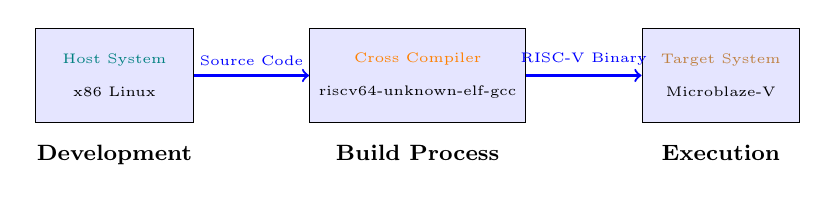
\begin{tikzpicture}[
    scale=0.7,
    box/.style={rectangle, draw, fill=blue!10, minimum width=2cm, minimum height=1.2cm, align=center},
    arrow/.style={->, thick, blue}
]

% Host System
\node[box] (host) at (0,0) {{\color{teal}\tiny Host System}\\\tiny x86 Linux};
\node[below=0.15cm of host] {\footnotesize \textbf{Development}};

% Cross Compiler
\node[box] (compiler) at (5.5,0) {{\color{orange}\tiny Cross Compiler}\\\tiny riscv64-unknown-elf-gcc};
\node[below=0.15cm of compiler] {\footnotesize \textbf{Build Process}};

% Target System
\node[box] (target) at (11,0) {{\color{brown}\tiny Target System}\\\tiny Microblaze-V};
\node[below=0.15cm of target] {\footnotesize\textbf{Execution}};

% Arrows
\draw[arrow] (host.east) -- (compiler.west) node[midway, above] {\tiny Source Code};
\draw[arrow] (compiler.east) -- (target.west) node[midway, above] {\tiny RISC-V Binary};

\end{tikzpicture}
\end{center}

\textbf{Why cross-compile?}
\begin{itemize}
    \item Target has different CPU architecture (RISC-V vs x86)
    \item Target has limited resources (memory, storage)
    \item Target may not have development tools
    \item Enables development on powerful host systems
\end{itemize}
\end{frame}

\begin{frame}
\frametitle{Meet the MicroBlaze-V}
\begin{columns}[T]
\begin{column}{0.6\textwidth}
\textbf{Microblaze-V Specifications:}
\begin{itemize}
    \item \footnotesize \textbf{CPU:} RISC-V RV32IMAFC soft core
    \item \footnotesize \textbf{Memory:} 128KB BRAM + DDR support
    \item \footnotesize \textbf{Implementation:} FPGA fabric (Zynq, Kintex, Virtex)
    \item \footnotesize \textbf{Peripherals:} UARTlite, Timer, Ethernet, GPIO, I2C, SPI
    \item \footnotesize \textbf{Toolchain:} Standard RISC-V GCC
    \item \footnotesize \textbf{Development:} QEMU emulation support
\end{itemize}
\end{column}
\begin{column}{0.4\textwidth}
\textbf{Perfect for validation because:}
\begin{itemize}
    \item \footnotesize Real RISC-V architecture
    \item \footnotesize Hardware peripherals
    \item \footnotesize Easy programming
    \item \footnotesize Low cost
    \item \footnotesize Excellent documentation
    \item \footnotesize Active community
\end{itemize}
\end{column}
\end{columns}

\vspace{0.5cm}
\begin{center}
\textbf{This is your validation hardware platform!}
\end{center}
\end{frame}

\begin{frame}[fragile]
\frametitle{Microblaze-V Development Environment}
\textbf{What is Microblaze-V?}
\begin{itemize}
    \item AMD's RISC-V based soft processor core
    \item Drop-in replacement for classic Microblaze
    \item RISC-V RV32IMAFC instruction set
    \item QEMU emulation support for development
    \item Standard RISC-V toolchain compatibility
\end{itemize}

\textbf{Project structure:}
\begin{lstlisting}[basicstyle=\fontsize{6}{6}\selectfont\ttfamily]
microblaze-v-project/
+-- src/
|   +-- start.s          # Assembly startup file
|   +-- main.c           # Main C program
|   +-- validation.c     # Validation functions
|   +-- peripherals.c    # Peripheral drivers
+-- include/
|   +-- peripherals.h    # Header files
+-- linker/
|   +-- microblaze_v.ld  # Linker script
+-- Makefile             # Build configuration
\end{lstlisting}
\end{frame}

\begin{frame}[fragile]
\frametitle{Makefile Configuration for Microblaze-V}
\textbf{Makefile for embedded project:}
\begin{lstlisting}[basicstyle=\fontsize{5}{6}\selectfont\ttfamily]
# Microblaze-V Validation Suite Makefile

# Toolchain
CC = riscv64-unknown-elf-gcc
OBJDUMP = riscv64-unknown-elf-objdump
OBJCOPY = riscv64-unknown-elf-objcopy

# Flags
CFLAGS = -march=rv32imafc -mabi=ilp32f -nostdlib -Iinclude
LDFLAGS = -T linker/microblaze_v.ld

# Directories
SRCDIR = src
INCDIR = include
BUILDDIR = build

# Source files
ASM_SOURCES = $(SRCDIR)/start.s
C_SOURCES = $(SRCDIR)/main.c $(SRCDIR)/validation.c \
            $(SRCDIR)/peripherals.c $(SRCDIR)/gpio_tests.c

# Object files
ASM_OBJECTS = $(ASM_SOURCES:$(SRCDIR)/%.s=$(BUILDDIR)/%.o)
C_OBJECTS = $(C_SOURCES:$(SRCDIR)/%.c=$(BUILDDIR)/%.o)
OBJECTS = $(ASM_OBJECTS) $(C_OBJECTS)

# Target
TARGET = $(BUILDDIR)/validation_suite

all: $(TARGET)

$(TARGET): $(BUILDDIR) $(OBJECTS)
	$(CC) $(CFLAGS) $(LDFLAGS) -o $@ $(OBJECTS)

$(BUILDDIR)/%.o: $(SRCDIR)/%.c
	$(CC) $(CFLAGS) -c $< -o $@

$(BUILDDIR)/%.o: $(SRCDIR)/%.s
	$(CC) $(CFLAGS) -c $< -o $@

$(BUILDDIR):
	mkdir -p $(BUILDDIR)

clean:
	rm -rf $(BUILDDIR)
\end{lstlisting}
\end{frame}

\begin{frame}[fragile]
\frametitle{Cross-Compilation Workflow}
\textbf{Build process:}
\begin{verbatim}
# 1. Build the project
make

# 2. Clean build files
make clean

# 3. Run in QEMU
make run

# 4. View disassembly
make disasm

# 5. Result files:
# build/validation_suite  - Executable for QEMU
# Can generate .bin and .hex with objcopy if needed
\end{verbatim}

\textbf{Running on Microblaze-V QEMU:}
\begin{enumerate}
    \item Build the project with \texttt{make}
    \item Launch QEMU with \texttt{make run}
    \item Program loads at address 0x00000000
    \item Monitor output via serial console
\end{enumerate}
\end{frame}

\begin{frame}[fragile]
\frametitle{Assembly Startup and Linker Script}
\textbf{Assembly startup file (src/start.s):}
\begin{lstlisting}[language={[x86masm]Assembler}, basicstyle=\fontsize{6}{6}\selectfont\ttfamily]
.section .text
.global _start

_start:
    # Set up stack pointer
    la sp, _stack_top

    # Jump to main C function
    call main

    # If main returns, infinite loop
1:  j 1b

.section .bss
.align 4
stack:
    .space 4096
_stack_top:
\end{lstlisting}

\textbf{Linker script (linker/microblaze\_v.ld):}
\begin{lstlisting}[basicstyle=\fontsize{6}{6}\selectfont\ttfamily]
MEMORY \{
    BRAM : ORIGIN = 0x00000000, LENGTH = 128K
\}

SECTIONS \{
    .text : \{ *(.text) *(.text.*) \} > BRAM
    .rodata : \{ *(.rodata) *(.rodata.*) \} > BRAM
    .data : \{ *(.data) *(.data.*) \} > BRAM
    .bss : \{ *(.bss) *(.bss.*) *(COMMON) \} > BRAM

    \_stack\_top = ORIGIN(BRAM) + LENGTH(BRAM);
\}
\end{lstlisting}
\end{frame}

\begin{frame}[fragile]
\frametitle{Validation Example: GPIO Testing}
\begin{lstlisting}[language=C, basicstyle=\fontsize{6}{6}\selectfont\ttfamily]
#include "peripherals.h"
#include <stdint.h>

#define GPIO_BASE        0x40000000
#define TEST_PIN_START   0
#define TEST_PIN_COUNT   8

typedef struct {
    uint8_t pin;
    int test_passed;
    char result_msg[64];
} gpio_test_result_t;

int test_gpio_pin(uint8_t pin) {
    volatile uint32_t *gpio_data = (volatile uint32_t *)GPIO_BASE;
    volatile uint32_t *gpio_tri = (volatile uint32_t *)(GPIO_BASE + 0x04);

    // Configure pin as output
    *gpio_tri &= ~(1 << pin);

    // Test high output
    *gpio_data |= (1 << pin);
    delay_ms(10);
    int high_read = (*gpio_data >> pin) & 1;

    // Test low output
    *gpio_data &= ~(1 << pin);
    delay_ms(10);
    int low_read = (*gpio_data >> pin) & 1;

    // Validation: high should read 1, low should read 0
    return (high_read == 1) && (low_read == 0);
}

int run_gpio_validation_suite(gpio_test_result_t results[]) {
    int passed_tests = 0;

    uartlite_puts("Starting GPIO validation suite...\n");

    for (int i = 0; i < TEST_PIN_COUNT; i++) {
        uint8_t pin = TEST_PIN_START + i;
        results[i].pin = pin;
        results[i].test_passed = test_gpio_pin(pin);

        if (results[i].test_passed) {
            uartlite_puts("Pin ");
            uartlite_putc('0' + pin);
            uartlite_puts(": PASS\n");
            passed_tests++;
        } else {
            uartlite_puts("Pin ");
            uartlite_putc('0' + pin);
            uartlite_puts(": FAIL\n");
        }

        // Brief delay between tests
        delay_ms(100);
    }

    return passed_tests;
}
\end{lstlisting}
\end{frame}

\begin{frame}
\frametitle{Embedded vs Desktop Programming}
\begin{center}
\begin{tabular}{|l|l|l|}
\hline
\textbf{Aspect} & \textbf{Desktop} & \textbf{Embedded} \\
\hline
Memory & GBs available & KBs available \\
Storage & GBs/TBs & KBs/MBs \\
OS & Full OS (Linux/Windows) & Bare metal/RTOS \\
Libraries & Full standard library & Limited stdlib \\
Debugging & GDB, IDE debuggers & Hardware debuggers \\
I/O & Files, network, GUI & GPIO, UART, SPI \\
Performance & Less critical & Highly optimized \\
Power & Unlimited & Battery constrained \\
\hline
\end{tabular}
\end{center}

\vspace{0.5cm}
\textbf{Embedded programming considerations:}
\begin{itemize}
    \item Memory usage optimization
    \item Real-time constraints
    \item Hardware-specific code
    \item Power management
    \item Reliability and fault tolerance
\end{itemize}
\end{frame}

\begin{frame}[fragile]
\frametitle{Portable Code Design}
\textbf{Hardware abstraction example:}
\begin{lstlisting}[language=C]
// hardware_abstraction.h
#ifdef MICROBLAZE_V_BUILD
    #include "peripherals.h"
    #define HAL_GPIO_WRITE(pin, value) gpio_write(pin, value)
    #define HAL_GPIO_READ(pin) gpio_read(pin)
    #define HAL_DELAY_MS(ms) delay_ms(ms)
#else
    // Desktop simulation
    #include <stdio.h>
    #include <unistd.h>
    extern int sim_gpio_state[];
    #define HAL_GPIO_WRITE(pin, value) (sim_gpio_state[pin] = value)
    #define HAL_GPIO_READ(pin) (sim_gpio_state[pin])
    #define HAL_DELAY_MS(ms) usleep((ms) * 1000)
#endif

// Your validation code uses HAL functions
void blink_status_led(void) {
    HAL_GPIO_WRITE(LED_PIN, 1);
    HAL_DELAY_MS(500);
    HAL_GPIO_WRITE(LED_PIN, 0);
    HAL_DELAY_MS(500);
}
\end{lstlisting}
\end{frame}

\begin{frame}[fragile]  % <- Add this [fragile] option
\frametitle{Static vs Dynamic Memory}
\textbf{Embedded systems prefer static allocation:}

\begin{columns}
\begin{column}{0.5\textwidth}
\textbf{Static (Good):}
\begin{lstlisting}[language=C]
// Fixed-size arrays
int test_results[MAX_TESTS];

// Static structures
ChipState chips[NUM_CHIPS];

// Stack variables
void test_function() {
    int local_var = 42;
    // ...
}
\end{lstlisting}
\end{column}
\begin{column}{0.5\textwidth}
\textbf{Dynamic (Avoid):}
\begin{lstlisting}[language=C]
// Heap allocation
int *results = malloc(
    sizeof(int) * num_tests);

// Variable-length arrays
void test_function(int n) {
    int array[n];  // Risky!
    // ...
}
\end{lstlisting}
\end{column}
\end{columns}

\vspace{0.5cm}
\textbf{Why avoid dynamic allocation?}
\begin{itemize}
    \item Limited heap space
    \item Memory fragmentation
    \item Unpredictable timing
    \item Risk of memory leaks
    \item No virtual memory protection
\end{itemize}
\end{frame}

\begin{frame}
\frametitle{Interactive Poll: Architecture Quiz}
\begin{center}
\Large Which is better for embedded validation?
\end{center}

\textbf{Scenario:} Testing 100 registers repeatedly

\textbf{Option A:} \texttt{int results[100];}

\textbf{Option B:} \texttt{int *results = malloc(100 * sizeof(int));}

\pause

\begin{alertblock}{Answer}
\textbf{Option A} - Static allocation is predictable and reliable!
\end{alertblock}

\vspace{0.5cm}
\textbf{Embedded rule:} If you can predict the size, use static allocation.
\end{frame}

\begin{frame}[fragile]
\frametitle{Function Organization Best Practices}
\textbf{Layered architecture for validation:}
\begin{lstlisting}[language=C]
// Layer 1: Hardware abstraction
void hal_gpio_init(uint8_t pin);
void hal_gpio_write(uint8_t pin, bool value);
bool hal_gpio_read(uint8_t pin);

// Layer 2: Device drivers
void led_init(void);
void led_on(void);
void led_off(void);
void led_blink(uint32_t duration_ms);

// Layer 3: Test primitives
int test_gpio_output(uint8_t pin);
int test_gpio_input(uint8_t pin);
int test_voltage_range(float voltage);

// Layer 4: Test suites
int run_gpio_test_suite(void);
int run_power_test_suite(void);
int run_complete_validation(void);

// Layer 5: Application
int main(void);
\end{lstlisting}
\end{frame}

\begin{frame}
\frametitle{Lab Preview: Cross-Compiled Validator}
\textbf{This afternoon you'll build:}
\begin{itemize}
    \item Modular validation library with headers
    \item Cross-compilation setup for Microblaze-V
    \item Makefile build configuration
    \item GPIO-based hardware testing
    \item Portable code that runs on both desktop and Microblaze-V
    \item AI-assisted optimization and debugging
\end{itemize}

\vspace{0.5cm}
\textbf{Deliverables:}
\begin{itemize}
    \item \texttt{validation.h} and \texttt{validation.c}
    \item \texttt{Makefile} for cross-compilation
    \item Working \texttt{.elf} file for Microblaze-V
    \item Desktop simulation version
    \item Documentation of build process
\end{itemize}
\end{frame}

\begin{frame}
\frametitle{Troubleshooting Cross-Compilation}
\textbf{Common issues and solutions:}

\begin{itemize}
    \item \textbf{SDK not found:} Check \texttt{MICROBLAZE\_SDK\_PATH} environment variable
    \item \textbf{Compiler errors:} Verify \texttt{riscv64-unknown-elf-gcc} installation
    \item \textbf{Make fails:} Check Makefile syntax and dependencies
    \item \textbf{Linking errors:} Check library dependencies in Makefile
    \item \textbf{QEMU fails:} Check QEMU Microblaze-V machine support
\end{itemize}

\vspace{0.5cm}
\textbf{Debug strategy:}
\begin{enumerate}
    \item Start with simple blink example
    \item Add complexity incrementally
    \item Use printf for debugging (via UART)
    \item Test on desktop first, then cross-compile
    \item Keep backup of working versions
\end{enumerate}
\end{frame}

\begin{frame}
\frametitle{Key Takeaways - Day 4}
\begin{itemize}
    \item \textbf{Modular design scales:} Header files enable code reuse
    \item \textbf{Cross-compilation opens doors:} Same code, different targets
    \item \textbf{Microblaze-V is powerful:} Real RISC-V platform for validation
    \item \textbf{Make manages complexity:} Automated build processes
    \item \textbf{Static allocation is safer:} Predictable memory usage
    \item \textbf{Layered architecture works:} Organize by abstraction level
\end{itemize}

\vspace{0.5cm}
\begin{center}
\textbf{You're now an embedded systems developer!}
\end{center}
\end{frame}

\begin{frame}
\frametitle{Tonight's Homework}
\textbf{Optimize your cross-compiled validator:}
\begin{enumerate}
    \item Refactor code into multiple source files
    \item Create comprehensive header documentation
    \item Optimize for embedded constraints (memory, speed)
    \item Add error handling and recovery
    \item Use AI to suggest performance improvements
    \item Test both desktop and embedded versions
\end{enumerate}

\vspace{0.5cm}
\textbf{Advanced challenges:}
\begin{itemize}
    \item Implement hardware abstraction layer
    \item Add configuration management
    \item Create automated test reporting
    \item Explore Microblaze-V SDK advanced features
\end{itemize}
\end{frame}

\begin{frame}
\frametitle{Tomorrow Preview: Hardware Debugging}
\begin{center}
\Large Real Hardware, Real Debugging!
\end{center}

\textbf{Day 5 topics:}
\begin{itemize}
    \item Advanced GDB techniques for embedded systems
    \item Microblaze-V peripheral programming (ADC, timers, UART)
    \item Hardware-in-the-loop testing concepts
    \item Fault injection and detection methods
    \item Real-time debugging strategies
    \item Performance optimization techniques
\end{itemize}

\vspace{0.5cm}
\begin{alertblock}{Hardware Day}
Tomorrow you'll be programming real silicon!
\end{alertblock}
\end{frame}

\begin{frame}
\frametitle{Questions \& Discussion}
\begin{center}
\Large Ready for embedded development?
\end{center}

\begin{itemize}
    \item Cross-compilation setup questions?
    \item Makefile configuration challenges?
    \item Modular programming concepts unclear?
    \item Microblaze-V hardware questions?
    \item Excited about tomorrow's hardware programming?
\end{itemize}

\vspace{1cm}
\begin{center}
\textbf{Time to build your first embedded validator!}
\end{center}
\end{frame}

\end{document}

